\subsection{Structural Responses to Bounded Relaxation}
  \label{subsec:structural-interpretation-projective-thermodynamics}

  Physical observables arise through a generically non-injective projection
  $\Pi : \Omega \rightarrow O$ from the relational substrate $\Omega$.
  The $\chi$ substrate evolves under a bounded relaxation flux,
  characterized by a Born--Infeld-type constraint $b_{\mathrm{BI}}$.
  This bound limits the admissible transfer of relational relaxation
  and prevents divergence of effective observables.

  When the relaxation flux approaches its admissible bound,
  the projection enters a saturation regime.
  In such regimes, distinct underlying configurations
  become structurally indistinguishable at the level of $O$.
  This loss of distinguishability induces an objective structural entropy
  associated with the projection:
  \begin{equation}
    S_{\Pi} = -\sum_{o \in O}
    \mu(\Pi^{-1}(o)) \log \mu(\Pi^{-1}(o)),
  \end{equation}
  which reflects non-injectivity rather than epistemic uncertainty.

  The relationship between the fluctuation amplitude and the relaxation flux defines
  a hierarchy of five regimes, ranging from the irreducible projective floor to the
  inadmissible regime beyond the Born--Infeld ceiling.
  Table~\ref{tab:fluctuation-hierarchy} provides an overview; each level is developed
  in the paragraphs below.

  \begin{table}[ht]
    \centering
    \begin{tabular}{clll}
      \hline
      \textbf{Level} & \textbf{Regime}         & \textbf{Mechanism}                 & \textbf{Example}
      \\
      \hline
      1              & Irreducible floor       & Minimal projective variance        & Zero-point energy
      $\tfrac{1}{2}\hbar\omega$ \\
      2              & Normal fluctuations     & $\lambda$-induced fibre drift      & Vacuum fluctuations
      \\
      3A             & Saturation (incoherent) & Thermodynamic compensation         & Solar corona heating
      \\
      3B             & Saturation (coherent)   & Coherent projective reorganisation & Superconductivity
      \\
      4              & Beyond BI ceiling       & Pair creation as dissipation       & Schwinger effect
      \\
      \hline
    \end{tabular}
    \caption{Hierarchy of projective fluctuation regimes.
    Levels~1 and~4 are structural boundaries: Level~1 is the irreducible floor below
    which temporal ordering ceases, Level~4 is the inadmissible ceiling above which
    admissibility is restored by pair creation.
    Levels~3A and~3B are alternative responses to the same saturation constraint,
      selected by the coherence of the projected fiber.}
    \label{tab:fluctuation-hierarchy}
  \end{table}

  \paragraph{Level~1 --- Irreducible projective floor.}

    The Born--Infeld bound does not only cap fluctuation amplitudes from above; it also
    implies a minimum below which the projection loses its capacity to generate
    distinguishable successive effective states.
    This floor corresponds to the minimal projective variance required to maintain
    $U_{n+1} \neq U_n$: the irreducible resolution limit of~$\Pi$.
    In the effective description, it manifests as the zero-point energy~$\tfrac{1}{2}\hbar\omega$
    of each mode---not as a physical excitation of the substrate, but as the smallest
    fluctuation amplitude consistent with a non-stationary projected description.
    A projection operating exactly at this floor would be locally injective and temporally
    stationary; as established in Section~\ref{subsec:structural-predictions-fluctuations},
    global stationarity is structurally excluded.

  \paragraph{Level~2 --- Normal fluctuation regime.}

    Above the floor, the projection operates in the normal fluctuation regime, governed
    by the $\lambda$-induced fibre drift mechanism developed in
    Section~\ref{subsec:projective-origin-of-fluctuations}.
    Two mechanisms contribute: fibre decorrelation, in which successive fibre slices
    become uncorrelated without amplitude growth, and projective amplification, in which
    residual norms grow under unstable directions of the relaxation dynamics~$F$.
    Both remain bounded by~$A^{\mathrm{BI}}_{\max}$.
    This regime accounts for the standard phenomenology of quantum vacuum fluctuations,
    including the Casimir effect (Section~\ref{subsec:casimir-effect})
    and projective spectral noise effects such as the Lamb shift~\cite{Beau2026f}.

  \paragraph{Level~3A --- Thermodynamic compensation.}

    In incoherent or weakly correlated systems,
    collective stabilization of the fiber is not available.
    The unresolved relational flux is therefore absorbed into
    effective thermodynamic descriptors.
    Temperature acts as a Lagrange multiplier compressing
    unresolved relational structure into the observable sector.

    Magnetically guided dilute plasmas, such as the solar corona, illustrate this regime.
    Reduced projectability under strong magnetic structuring
    leads to an elevated effective temperature,
    interpretable as a compensatory response to bounded relaxation
    rather than as excess local energy density.

  \paragraph{Level~3B --- Coherent reorganization.}

    In strongly coherent collective phases,
    the system may instead reorganize its internal fiber structure
    so as to preserve maximal projective stability.
    Rather than inflating thermodynamic variables,
    the projected description modifies its admissible connection structure.

    Superconductivity provides a paradigmatic example.
    Collective phase locking of the $U(1)$ fiber
    suppresses internal fluctuations and enforces
    near-vanishing covariant phase gradients in the bulk.
    The Meissner effect may therefore be interpreted
    as the expulsion of incompatible connection curvature,
    maintaining projective stability within the coherent phase.

  \paragraph{Level~4 --- Beyond the Born--Infeld ceiling.}

    When the relaxation flux exceeds the admissible bound~$b_{\mathrm{BI}}$,
    the projection enters an inadmissible regime: no stable effective description can
    be maintained at the current flux level.
    Admissibility is restored by a structural reconfiguration of the projection fiber,
    manifesting in the effective description as the creation of particle--antiparticle pairs.
    Pair creation thus acts as a dissipative channel that redistributes excess relational
    flux into stable, projectable modes, enlarging the space of admissible configurations
    and restoring the projection below the Born--Infeld ceiling.
    The Schwinger effect---spontaneous pair production in ultra-strong electric
    fields~\cite{Beau2026f}---is the paradigmatic instance of this regime.
    It emerges here not from vacuum fluctuations or Dirac-sea arguments, but as a
    universal transition between smooth relaxation and topologically mediated dissipation.

  \paragraph{Unified interpretation.}

    These five levels do not represent distinct physical mechanisms but a single
    continuous structural response to the bounded relaxation constraint, resolved
    differently depending on the amplitude of the flux, the coherence of the fiber,
    and the dynamical accessibility of collective reorganization.

    Thermodynamic variables, geometric curvature, horizon formation, and collective
    coherence all act as compensatory descriptors of unresolved relational structure.
    Which response occurs depends on whether collective reorganization of the projected
    fiber is dynamically accessible.

    The bounded character of substratic relaxation ensures that projection-induced
    thermodynamic and geometric quantities remain finite.
    This renders the framework predictive despite the intrinsic non-injectivity of~$\Pi$,
    and replaces the ultraviolet divergences of standard quantum field theory---controlled
    there by renormalisation---with a structurally motivated finite ceiling grounded in
    the Born--Infeld admissibility constraint.

    \begin{figure}[t]
      \centering
      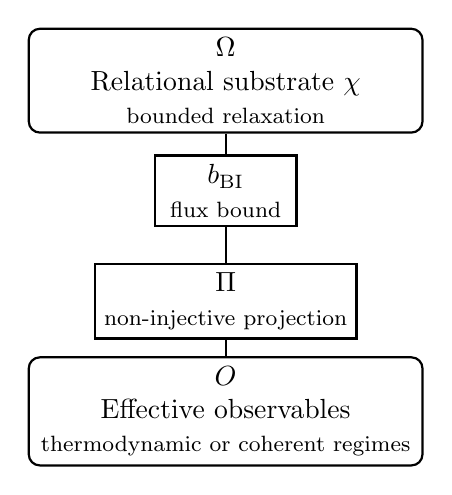
\begin{tikzpicture}[
        node distance=1.4cm,
        every node/.style={align=center},
        box/.style={draw, rounded corners, thick,
        minimum width=5cm, minimum height=1cm},
        narrow/.style={draw, thick,
        minimum width=1.8cm, minimum height=0.8cm}
      ]
        \node[box] (omega)
        {$\Omega$\\Relational substrate $\chi$\\
        {\footnotesize bounded relaxation}};
        \node[narrow, below of=omega] (bi)
        {$b_{\mathrm{BI}}$\\
        {\footnotesize flux bound}};
        \node[narrow, below of=bi] (pi)
        {$\Pi$\\
        {\footnotesize non-injective projection}};
        \node[box, below of=pi] (obs)
        {$O$\\Effective observables\\
        {\footnotesize thermodynamic or coherent regimes}};
        \draw[thick] (omega) -- (bi);
        \draw[thick] (bi) -- (pi);
        \draw[thick] (pi) -- (obs);
      \end{tikzpicture}
      \caption{Structural responses to bounded relaxation.
      Approach to the flux bound may induce either compensatory
      thermodynamic descriptors or coherent projective reorganization,
        depending on collective accessibility of the fiber structure.}
      \label{fig:projective-hourglass}
    \end{figure}
